\chapter{马克思论信用制度(第三卷 第27—37章)}

几经尝试后,恩格斯放弃了重建马克思《混乱》中的观点,最终他将自身的努力仅限于复制马克思的笔记,并强调了一些他临时做出的批判性补充。……我想先对我所理解的总体脉络做一个综述。必须澄清的是,我这样做并非是要声称我的解读是唯一可能的,更不用说是唯一正确的。

它将货币资本循环看作是一种中枢神经系统,引导了实现总体资本再生产的资本流动。此外,
它意味着一种资本的社会化——标志着资本特征的一些根本改变。例如,股份公司有利于集体、
联合资本的出现,一方面允许了资本主义在规模、范围以及形式上的巨大扩展,另一方面为
资本主义开辟了一条通往世界市场的道路,在世界市场里联合劳动和集体产权会得到更快的
发展。马克思甚至认为股份公司会由于其联合的特性而成为向非资本主义生产方式过渡的基
础。这个观点在现在看来即便不是错误的,也是很奇怪的,但在他那个时代确实存在一些有
趣的原因使人考虑这种可能性。(Note)

圣西门想要给国王提供建议,于是他给国王寄了很多书信,提出了改善集体生活的各种途径,以避免他所极度厌恶的像法国大革命那样的暴力变革。圣西门大概是最早提出欧盟之类想法的思想家之一。假如人们听从了他的建议,两次世界大战也许是可以避免的。他提出政府应该具有合理性和代表性,从而在仁慈的君主制度下可以通过立法保证所有阶级的利益。他还强调了将资本和劳动力(包括手工艺人和资本主义企业家)结合起来以建造有助于提高每个人福利的大规模(一定程度上是有计划的)项目和市政工程的重要性。为了使之变为现实,就需要将分散在社会中的以浪费形式存在的小量货币资本以联合的形式集中起来。

\begin{quotation}
货币主义本质上是天主教的;信用主义本质上是基督教的。“苏格兰人讨厌金子”。作为纸币,商品的货币存在只是一种社会存在。信仰使人得救。这是对作为商品内在精神的货币价值的信仰,对生产方式及其预定秩序的信仰,对只是作为自行增殖的资本的人格化的各个生产当事人的信仰。但是,正如基督教没有从天主教的基础上解放出来一样,信用主义也没有从货币主义的基础上解放出来。\pagescite[][670]{capital3} (Note)

正是信用和银行制度的发展,一方面迫使所有货币资本为生产服务(也就是说,使所有货币收入转化为资本),另一方面又在周期的一定阶段,使金属准备减少到最低限度,使它不再能执行它应该执行的职能。正是这种发达的信用制度和银行制度,引起了整个机体的这种过敏现象。\pagescite[][648]{capital3} (Big Note)


\end{quotation}

\begin{figure}
\centering
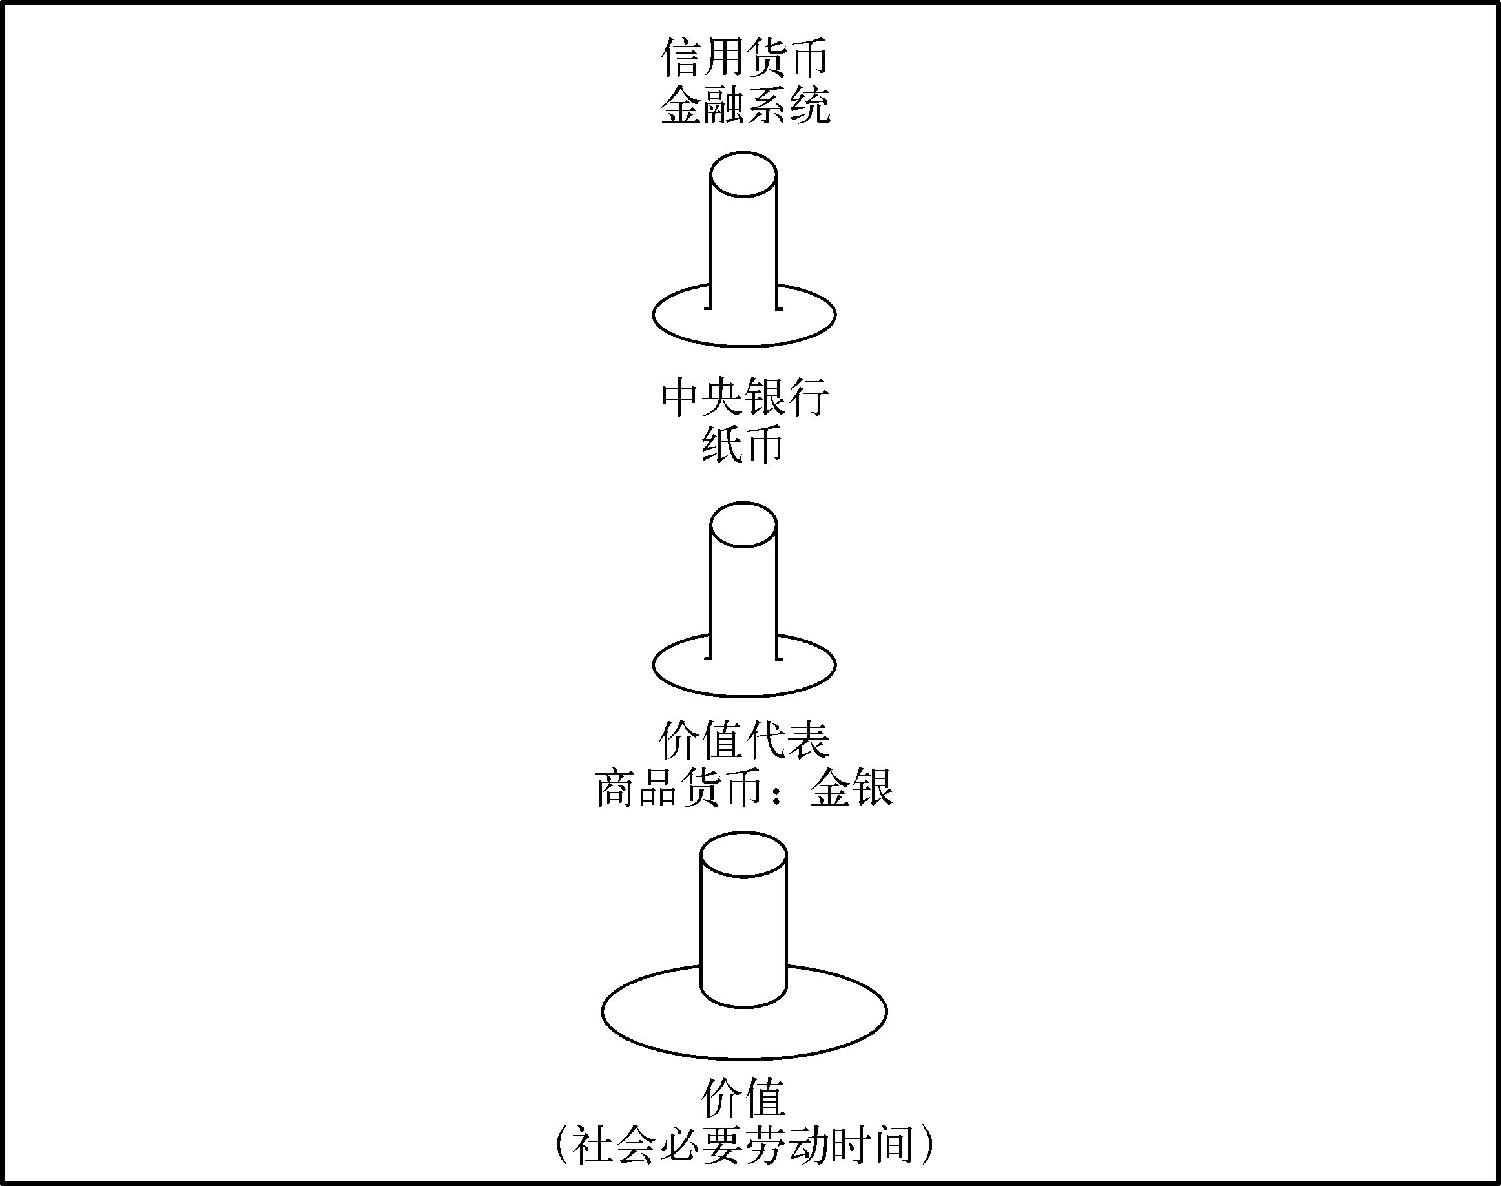
\includegraphics[scale=0.3]{david4.jpg}
\caption{马克思的等级制货币体系}
\label{fig:david4}
\end{figure}

尽管连全球信用和货币体系中徒有其表的金属或商品基础在20世纪70年代早期就被废除了
(虽然所谓的主张回归金本位的人还很多),全球金融体系枢纽(以美元为中心)的等级制
结构设想貌似依旧是合适的。我们比马克思活着的时候更接近这样一种现实:

\begin{quotation}
  同样作为财富的社会形式的信用,排挤货币,并篡夺它的位置。正是由于对生产社会性质
  的信任,才使得产品的货币形式表现为某种转瞬即逝的和观念的东西,表现为单纯想像的
  东西。

  但是,一当信用发生动摇,——而这个阶段总是必然地在现代产业周期中出现,——一切现实
  的财富就都会要求现实地、突然地转化为货币,转化为金和银。这是一种荒谬的要求,但
  是它必然会由这个制度本身产生出来。而应当能够满足这种巨大要求的全部金银,不过是
  银行地库里的几百万镑。\pagescite[][650]{capital3} (Big Big Note)

\end{quotation}

那么当信用货币和信用业务取代了商品货币之后会发生什么呢?第一,“在信用收缩或完全
停止的紧迫时期,货币会突然作为惟一的支付手段和真正的价值存在,绝对地同商品相对立。
因此,商品会全面跌价,并且难于甚至不可能转化为货币,就是说,难于甚至不可能转化为
它们自己的纯粹幻想的形式”。这里确切体现了拜物教理论。第二,“信用货币本身只有在
它的名义价值额上绝对代表现实货币时,才是货币”。当金流向国外时,信用兑换成货币的
可能性,即它和现实的金的同一性,就成问题了。为了保证这种兑换的条件,就采取各种强
制性的措施,提高利息率等等。……信用货币的贬值(更不用说它的只是幻想的货币资格的
丧失)会动摇一切现有的关系。因此,为了保证商品价值在货币上的幻想的、独立的存在,
就要牺牲商品的价值……因此,为了几百万货币,必须牺牲许多百万商品。这种现象在资本
主义生产中是不可避免的,并且是它的妙处之一……一旦劳动的社会性质表现为商品的货币
存在,从而表现为一个处于现实生产之外的东西,货币危机——与现实危机相独立的货币危机,
或作为现实危机尖锐化表现的货币危机——就是不可避免
的。\pagescite[][584-585]{capital3} (Big Big Note)

这就是20世纪30年代大萧条中发生的事情吗?这就是凯恩斯主义努力去纠正的“不可避免的”的问题吗?

\begin{quotation}
  这种情况之所以在资本主义体系内表现得最为尖锐,并且以矛盾百出、荒唐可笑的形式表
  现出来,是因为1. 在资本主义体系中,为直接的使用价值,为生产者本人的需要而进行的
  生产,已经完全废止,因此,财富只是作为社会过程而存在,这个社会过程表现为生产和
  流通的错综交织;2. 随着信用制度的发展,资本主义生产不断地企图突破对财富及其运动
  的这个金属的限制,\textbf{突破这个物质的同时又是幻想的限制,但又不断地在这个限制面前碰
  破头。}\pagescite[][650]{capital3}(Big Big Note)

\end{quotation}

马克思认为,纯粹基于商品货币的货币体系将会成为资本进一步积累的障碍,这是因为金的
数量满足不了需求。我们现在所谓的“金融抑制”是一个明显的、持续的危险,当货币(任
何种类)的数量不足以支撑资本积累带来的持续扩大的商品量流通时,这种“金融抑制”就
会出现。因此信用货币不但对资本主义的持续扩张是必需的,而且是至关重要的。有初步的
证据表明(虽然据我所知还没有经验研究)资本积累的历史是和信用货币的积累以及与其共
存的债务积累同步进行的。只有通过这种方式资本才能“\textbf{没有限制地}”进行积累。
但是如果资本积累取决于同时进行的信用货币和信用票据的积累,那么必定会产生一种基于
信念、信任和预期且会周期性突然失控的拜物教信仰。信用货币不是简单地代替贵金属货币:
他们会把货币体系和货币的概念带到一个全新的水平上,\textbf{会欢迎而不是揭穿在信用
  制度中所隐含的拜物教。}信用“泡沫”,资产泡沫,以及投机性的繁荣和萧条都是资本为
了将自己暂时地从货币—商品的限制中解放出来而必须付出的代价。(Big Big Note)

对信用制度至关重要的是,它具备冲破一切资本积累的货币障碍而无限制增长的能力。纸币
(欠条)的创造会导致无限制的可能性。美国2001年之后的房地产泡沫就是这样出现的。价
格在上升,每个人都从房价上涨中大赚一笔,而且他们赚得越多,价格就涨得越多。房子就
像ATM机一样,没有提取的限制,\textbf{直到人们意识到房地产的价格已经远远的超出了他们收入的
支付能力。}房地产市场的崩溃接踵而来。20世纪80年代日本的土地投机热潮破灭之后发生了
相同的事情。当崩溃来临时,所有者(掌控着硬通货)的资产流动性才是最重要的。当人们
发现\textbf{流动性不足的时候,止赎、损失和资产贬值就越积越多}。(Big Big Note)

但是,如果整个货币体系中的贵金属“枢纽”消失了,那么什么会取代它成为枢纽呢?答案
就是\textbf{世界央行和国家监管当局两者的结合体(我把它称作“国家—金融联合体”)},
它们共同形成了全球货币和信用制度的枢纽。对于马克思而言,这种枢纽就是英格兰银行,
而对我们而言,就是美国联邦储备银行(和美国财政部)和世界其他央行及监管当局,比如
英国、日本和欧盟的央行。然而\textbf{它们的效果是,用人造的制度取代依赖于实际商品
  生产(金和银)的调节机制。人们的判断是信用创造的唯一规则。}但是,人造的制度能正
确发挥作用吗?我们必须转而关注央行的组织和调节,以及政策是如何由国家机构制定出来
以应对信用制度的周期性过剩的。(Big Big Note)

现在人们普遍认为管制失灵影响了最近的几起事件,也有人鼓吹美国乃至全球经济危机的解
决之道就在于建立一个更好的监管机制。但是,我们应该如何利用这样的一个欧洲央行
呢?\textbf{它以控制通货膨胀为唯一目标而不顾失业,}它面对希腊债务危机时束手无策,
仅仅推行紧缩政策使得希腊元气大伤并日益衰退。人造的制度是不可靠的,受制于各种社会
势力和矛盾意见。他们创造了一个大不相同的调节机制,和商品货币依然作为枢纽时的央行
相去甚远。

即便在马克思的时代,金融机构及其政策的不可靠性也扮演了很重要的角色。马克思把“错
误的”1844年英国银行法案作为最好的例子。这项立法把英格兰银行分为了“一个发行部和
一个银行部”。[12]前一个部门持有政府债券和金属储备,以此为储备金发行银行券。该部
门用银行券(对贸易极为便利)换取金,并承诺如果需要的话,银行可以“支付给持券
者”金(在英国的银行券上,依旧可以找到答应支付给持券者的语句)。因此,在任何时候,
我拿着银行券去银行就可以换金。简而言之,银行券是可兑换的(停止兑现往往是那时候的
政治选择,实际上拿破仑战争期间英国就曾经中止兑现金)。另一个部门则贴现票据,承兑
支票,发行债券并参与其他传统的银行业务。1844年的立法在银行的两部分之间创造了一堵
防火墙。但是在1848年,一场信用危机打击了银行部。人们对已贴现商业票据和债券失去了
信心,发生了银行挤兑。银行部用光了金,而发行部门却拥有大量的金:

左拉的小说《金钱》以萨加尔(贝列拉兄弟)和甘德曼(罗斯柴尔德家族)在第二帝国时期的斗争为中心,描写金融投机中人们情感与理智的冲突。下面是萨加尔说的一番话,他想要说服他严肃、高尚、好沉思的侄女卡洛琳娜夫人,改变她瞧不起他的投机活动的想法:

\begin{quotation}
“看这儿,”萨加尔喊道,“你将会看到这些无人区和荒芜道路的彻底的复兴,我们的铁路将会穿过这些地方——是的!当我们把新的血液注入到这个体系的干涸的血管里时,土地将被清整,道路和运河将被建造起来,新的城市将会破土而出,生活也会好起来的。是的!这就是货币带来的奇迹……”

“你一定要明白,投机、赌博就是核心,是心脏。是的,它从各个小支流中吸引、收集了血液,然后再在河流中把血液输送到各个方向,于是\textbf{形成了一个巨大的货币流通},这正是大企业的生命所在。”

“投机——为什么是我们所必须经历的刺激物?因为投机是强迫我们生活、奋斗的永恒的欲望。没有了投机,噢我亲爱的朋友,什么类型的买卖都会没有……投机和爱情是一样的。相爱和投机都充满了肮脏;相爱时人们也仅仅考虑他们自己的喜悦;但是没有爱情就没有生命,那么世界就将终结。”
\end{quotation}

读了这段文字,你就可以很容易地理解,为什么马克思在提到贝列拉时会说起他“既是骗子又是预言家”。


信用制度看上去是混乱和不受约束的,它酝酿投机热潮和周期性崩溃的能力不受限制。这是可以预见的,因为利息,用《政治经济学批判大纲》里的话来说,属于特殊性,并且由其他特殊性调节(如果可能的话)——比如货币的供给和需求,还有不同资本派系之间的竞争。因此,利息注定是偶然、不受约束和失常的。利息也取决于信念。

对于这种阶级关系的永恒存在来说,资本“白手起家”的神话可以有效地巩固资产阶级在意识形态上的合法地位,同时使资产阶级得到更新和保持活力。因此缺乏向上的流动性(或是向上的流动性减小,正如美国近期那样)往往被看作是不利于维护资本主义社会秩序的。就现代信用制度促进了这种向上的流动性和灵活性来说,它也有积极的一面。(Note)

\begin{quotation}
这种反高利贷的激烈斗争,这种让生息资本从属于产业资本的要求,只是这样一种有机创造物的先声,这种有机创造物以现代银行制度为形式创造了资本主义生产的这些条件。现代银行制度,一方面把一切闲置的货币准备金集中起来,并把它投入货币市场,从而剥夺了高利贷资本的垄断,另一方面又建立信用货币,从而限制了贵金属本身的垄断。\pagescite[][682]{capital3} 

但是,绝不要忘记,第一,货币——贵金属形式的货币——仍然是基础,信用制度按其本性来说
永远不能脱离这个基础。第二,\textbf{信用制度以社会生产资料(以资本和土地所有权的
  形式)在私人手里的垄断为前提,}所以,一方面,它本身是资本主义生产方式固有的形式,
另一方面,它又是促使资本主义生产方式发展到它所能达到的最高和最后形式的动
力。\pagescite[][685]{capital3}

\end{quotation}

马克思显然把话说得太死了,因为我们现在的货币体系就不是以贵金属为基础的。我们也许
要用\textbf{怀疑的态度}来看待这个列宁一个世纪前提出的目的论观点,即\textbf{金融资
  本是资本主义生产方式可以采取的最高级也是最后的可能形式}。虽然毫无疑问金融资本在
一些历史阶段上变得更为突出,甚至拥有霸权地位,但是我认为资本各部分之间的力量均衡
不会注定只向一个方向演变的。(Big Note)

但是我们现在已经处于这样一个阶段,货币和国家之间的“内在关系”已经变得如此紧密,
以至于\textbf{很难想象一个可以从外部对金融化进行调控的国家力量}。证据便是美国最近
的多德—弗兰克金融管制改革法案。这个法案基本上是由银行家写的,不仅实施得不清不楚,
而且每条每款都主要遵循了银行业游说集团的意志。但是,如果我的观点——国家—金融联合体
在资本主义历史中发挥了长期的作用——是对的,那么这种“内在关系”不过是使资本回到了
它的起源。那么,这究竟是意味着国家仅仅是资本的一种工具,还是意味着近年来国家和金
融(注意,只是金融,而不是一般意义上的资本)的融合已经变形成了某种本质上完全不同
的东西?确实,债券持有人现在对国家政策的公开影响力似乎比以前更大了。但是我还记得
哈罗德·威尔逊(20世纪60年代的英国工党首相)曾经抱怨“苏黎世侏儒”决定其经济政策的
力量,正如他让步于伦敦金融家的需求而牺牲英国生产资本的利益一样。这和比尔·克林顿著
名的失意的感叹相同。在他的首次就职典礼前,克林顿对他的经济顾问们说:“你们的意思
是说,我的经济政策和连任前景都要取决于一群该死的证券交易员的观点?”对于这个问题,
答案是:“的确如此!”我认为,我们对国家和金融的力量交织历史的了解,还没有精细到
足以判断我们现在是否处在不同的处境的地步,尽管我们确定地知道金融管制和金融制度改
革的问题现在已成为了国际问题,任何一个国家都不可能单凭一己之力解决。

但是马克思特别讨论了信用制度内部的“内在力量”将把我们引向哪里。“资本的这种社会
性质,只是在信用制度和银行制度有了充分发展时才表现出来并完全实现。……因此,信用
制度和银行制度扬弃了资本的私人性质,从而自在地,但仅仅也是自在的包含着资本本身的
扬弃。”这是一个相当惊人的叙述,但是我们将会看到,马克思在其他地方会重复提
起。“银行业和信用同时又成了使资本主义生产超出它本身界限的最有力的手段,也是引起
危机和欺诈行为的一种最有效的工具。”

\begin{quotation}
毫无疑问,在由资本主义的生产方式向联合起来劳动的生产方式过渡时,信用制度会作为有力的杠杆发生作用;但是,它仅仅是和生产方式本身的其他重大的有机变革相联系的一个要素。与此相反,关于信用制度和银行制度的奇迹般的力量的种种幻想所以会被赋予社会主义的意义,是由于对资本主义生产方式和作为它的形式之一的信用制度完全没有认识。\pagescite[][686]{capital3} 
\end{quotation}

\chapter{信用和银行系统的作用(第三卷 第27章开始)}

第27章,马克思列举了许多金融部门发挥的重要作用。总结如下:

1. 它促进了货币资本在部门和产业之间的顺畅流动,这样利润率到处都被平均化了。马克思
在此之前把信用的功能归为“阶级的共有资本”,我认为主要就是这个意思。资本的“蝴
蝶”形式不停地移动,使不同产业、活动和地区的收益率标准化。

2. 它显著地减少了(a) 流通费用——通过免除商品货币的使用,用纸币取代黄金和降低了为适应商品交换的波动而持有准备金(窖藏)的必要性,同时(b) 减少周转时间(或者“加速商品形态变化的速度”和加速“货币流通的速度”)。这种流通的加速通常会延伸到资本的再生产过程。总之,它促进了资本的加速(周转时间的分析很清楚地表明了这点)。

3. 它允许股份公司的成立,使可能的生产规模惊人地扩大了,允许以前的政府职能私有化,
并有助于集中资本(正如第一卷中提到的)。这意味着许多资本主义企业现在取得了和私有、
个人相对立的社会特征。马克思有些令人惊讶地推断:\textbf{“这是作为私人财产的资本
  在资本主义生产方式本身范围内的扬弃。”}它加强了这种转化——“实际执行职能的资本家
转化为单纯的经理,别人的资本的管理人,而资本所有者则转化为单纯的所有者,单纯的货
币资本家。”\pagescite[][495]{capital3}

\begin{quotation}
因为利润在这里纯粹采取利息的形式,所以那些仅仅提供利息的企业仍然可以存在;这是阻止一般利润率下降的原因之一,因为这些不变资本比可变资本庞大得多的企业,不一定参加一般利润率的平均化。\pagescite[][496]{capital3} (Big Note)

\end{quotation}

保罗·博卡拉(Paul Boccara),20世纪60年代末法国共产党的主要理论家,认为这是这些年
中阻碍利润率趋于下降的主要力量。\textbf{投资于大规模基础设施的资本(不论是由国家还是股份
公司融资)的确可以,而且一般也是以这种方式流通的——只要求利息,事实上补贴了其他地
方的利润。个别资本家也可以选择租用他们的大部分不变资本(比如叉式升降车和其他形式
的机械),从而节约了大量不变资本的费用(对他们而言)。他们只支付了以商品形式借贷
的资本的等值利息,而不是支付商品的全部价值(利息加利润)。} (Big Big Note)

现在,固定资本的物理量(physical mass)嵌入建成环境(这个物理量证明了生产中不变资
本与可变资本比率极大提高的观点)中,\textbf{这种固定资本的绝大部分主要不是通过相关商品的
直接买卖而是作为获取租金的生息资本进行循环。地租的榨取和生息资本流通(巨额的抵押
贷款市场的存在就是绝好的例证)之间的关系就成为资本主义动态中的重要特征。}这是一个
马克思几乎没有涉及的话题(尽管我们很快就会看到,抵押贷款被定义为“虚拟资本”的一
种形式)。(Big Big Note: 我们国家的城镇化策略是不是也这样呢?)

\begin{quotation}


它在一定部门中造成了垄断,因而引起国家的干涉。它再生产出了一种新的金融贵族,一种新的寄生虫,——发起人、创业人和徒有其名的董事;并在创立公司、发行股票和进行股票交易方面再生产出了一整套投机和欺诈活动。这是一种没有私有财产控制的私人生产。\pagescite[][497]{capital3} 

\end{quotation}
第二帝国时期巴黎风趣的评论者们说,资本和商业变成了“其他人的钱”,指的就是这种情况。这就是贝列拉兄弟构想的世界:圣西门的乌托邦成为反乌托邦。马克思指出的“金融贵族”在今天更加显要。

“信用为单个资本家或被当作资本家的人,提供在一定界限内绝对支配他人的资本,他人的
财产,从而他人的劳动的权利……对社会资本而不是对自己的资本的支配权,使他取得了对
社会劳动的支配权。”马克思认为这里涉及的社会化有巨大的潜在重要性。“一个人实际拥
有的或公众认为他拥有的资本本身,只是成为信用这个上层建筑的基础。”结果,“在这里,
一切尺度,一切在资本主义生产方式内多少还可以站得住脚的辩护理由都消失了。进行投机
的批发商人是拿社会的财产,而不是拿自己的财产来进行冒险的。资本起源于节约的说法,
也变成荒唐的了,因为那种人正是要求别人为他而节约”。\pagescite[][498]{capital3} (Big Big Note)

\begin{quotation}
在资本主义生产很不发达的阶段还有某种意义的各种观念,在这里变得完全没有意义了。在这里,成功和失败同时导致资本的集中,从而导致最大规模的剥夺。在这里,剥夺已经从直接生产者扩展到中小资本家自身。这种剥夺是资本主义生产方式的出发点;实行这种剥夺是资本主义生产方式的目的,而且最后是要剥夺一切个人的生产资料……这种剥夺在资本主义制度本身内,以对立的形态表现出来,即社会财产为少数人所占有;而信用使这少数人越来越具有纯粹冒险家的性质。因为财产在这里是以股票的形式存在的,所以它的运动和转移就纯粹变成了交易所赌博的结果;在这种赌博中,小鱼为鲨鱼所吞掉,羊为交易所的狼所吞掉。\pagescite[][498]{capital3} (Big Big Note)

\end{quotation}

他考察货币经营资本历史时要阐明的一般主题是,高利贷和利息必须被规训并服从于一般的
资本主义生产方式以及特殊的产业资本循环的要求。然而这些段落意味着资本主义信用制度
完全不受控制,以致它现在反而以有害的、扭曲的方式威胁到资本和剩余价值生产的世界。
它以掠夺式积累而不是在生产领域剥削劳动力为中心。它在经济中再次引入高利贷业务,尽
管和很久以前的高利贷完全不同。这会威胁到资本积累的持续性吗?马克思没有给出明确的
答案,但确实暗示了这种可能性。

\begin{quotation}


信用制度是资本主义的私人企业逐渐转化为资本主义的股份公司的主要基础,同样,它又是按或大或小的国家规模逐渐扩大合作企业的手段。资本主义的股份企业,也和合作工厂一样,应当被看作是由资本主义生产方式转化为联合的生产方式的过渡形式,只不过在前者那里,对立是消极地扬弃的,而在后者那里,对立是积极地扬弃的。\pagescite[][499]{capital3} 

\end{quotation}
马克思完成这一章的草稿后,恩格斯插入了几页来描述公司资本的力量的演化。可以推断出,恩格斯认为从这一切中建立任何进步事物的时机都早已过去了。恩格斯在其他地方写到,马克思非常尊敬圣西门的思想,即为了进步的目的运用联合起来的资本的力量。在这里,马克思美化了这个思想,并提出了通过工人的协同控制来管理联合起来的资本的前景。尽管他承认这些工人合作社注定会再生产出现存制度的许多缺点,但它们至少为通过合作运动和实践的传播来征服一个国家提供了一个依据。(Big Note)

这一问题很重要,因为当代许多正在进行的运动相信这一时机已经再次来临了——通过接管工
厂进行的生产的民主化,可选择的“团结经济”(Solidarity Economy)的发展,物物交换
网络和其他合作形式——它们本身就是一条通向一个彻底反资本主义的政治和经济生活重建的
道路。尽管许多参与者意识到,在合作社形式里,不仅自我剥削十分困难,而且不可避免地
再生产出了他们寻求取代的资本主义制度的很多缺陷,这条道路还是经常被描述为民主的反
资本主义运动的唯一选择。似乎信用制度的兴起和资本社会化提供了合作社和工人控制可能
兴盛的“自然”基础。然而,这里没有提到《共产党宣言》中把所有信用集中于工人控制的
国家手中的要求。

但是也有许多引人警戒的故事。前些年,皮奥里和萨贝尔写了一本颇有影响力的《第二次产
业革命》。他们提出,弹性专业化和小批量生产的新劳动实践,为工人控制的小规模合作生
产(如第三意大利的艾米利亚—罗马涅区所展示的)开辟了空间(和1848年存在的相似);这
种形式将打败公司主导的工厂生产形式,并提供转化到分散的社会主义的机制。[15]皮奥里
和萨贝尔发起了一场相当有效的运动(特别是在欧洲)来说服组织起来的工人放弃对新技术
和新组织形式的敌意,让他们像拥护自由解放一样拥护弹性专业化(他们非常迷恋蒲鲁东的
观点,当然这些观点是马克思不能容忍的)。皮奥里和萨贝尔没有意识到的是,弹性专业化
促进了灵活积累下的恶意剥削的实践,而灵活积累居于新自由主义计划的核心。弹性专业化
成为所有采用它的生产场所中规训和压制劳动力的主要手段。现在再没人亲切地说它能带来
解放了。\textbf{历史上很多事物看似蕴含着解放的可能性,结果却是资本主义剥削的支配性实践的
回归,这的确很令人悲哀。所以,当心你自己的愿望。}

从马克思的角度来看,更有意义的区别是货币被资本家用来购买用于生产的商品,还是被借来购买已经生产出来的商品。这个区别是“收入的货币形式和资本的货币形式之间的区别”。\pagescite[][503]{capital3} 两种货币的使用都包含在产业资本的流通中。马克思有时把流入生产的信用称为“货币资本”,与流向消费者支持市场中价值和剩余价值实现的“货币经营资本”相对立。

马克思仔细考察了当银行资本为了利息的回报而借出时会发生什么。他指出,利息可以看作
是任何收入流的等价物。如果利率是5\% ,那么“每一笔固定的二十五镑的年收入,都可以
看作五百镑资本的利息”。但马克思评论这是一种“纯粹幻想的观念”。收入流的后面不一
定要有任何实际的货币资本。比如,许多美国公民每月都会收到社会保险支票,但认为这笔
货币流是某些国家持有的资本的利息的想法是一种幻觉。然而,社会保险接受者如果承诺把
每年收到的二万五千美元交给银行,就可以获得五十万美元的货币资本来买房子。二万五千
美元的年收入被资本化为五十万美元,\textbf{即使社会保险金后面没有初始的货币资本量
  (只是国家提供每月收入的一种承诺,它以对工资征税的方式获得资金)。}这使我们考虑
马克思最重要的概念之一,虚拟资本。

\begin{quotation}
  但在这一切场合,这种资本,即把国家付款看成是自己的幼仔(利息)的资本,
  是\textbf{幻想的虚拟的资本}。…… 这个金额从来不是要作为资本支出的,不是要作为
  资本投下的,而只有作为资本投下,它才能转化为一个自行保存的价值。……不管这种交
  易反复进行多少次,国债的资本仍然是纯粹的虚拟资本;一旦债券不能卖出,这个资本的
  假象就会消失。然而,我们马上就会知道,这种虚拟资本有它的独特的运
  动。\pagescite[][527]{capital3}

生息资本一般是一切颠倒错乱形式之母。……资本家们思考方式的错乱在这里达到了顶点,资本的增殖不是用劳动力的被剥削来说明,相反,劳动力的生产性质却用劳动力本身是这样一种神秘的东西即生息资本来说明。\pagescite[][528]{capital3} 
\end{quotation}

马克思提到的“独特的运动”是那种我们看到的股票和债券市场每天甚至每小时的价值波动。
当资产阶级理论家把工资流归于劳动者并且创造出物化在工人身上的虚拟资本时,这种颠倒
错乱更显著地表现出来了。工人的价值就被计算为年工资的资本化价值。所以根据这个理论,
如果工人投资教育和获得技能,人力资本价值就可以提高,他将以更高工资的形式得到回报。
按照人力资本理论,工人是资本家!

所有这些背后有一个简单却关键的原则,即资本化:“人们把虚拟资本的形式叫作资本化。
人们把每一个有规则的会反复取得的收入按平均利息率来计算,把它算作是按这个利息率贷
出的一个资本会提供的收益。”这笔收益流的所有权证书可以按照这个资本化的价格交
易。“因此,和资本的现实增殖过程的一切联系就彻底消灭干净了。资本是一个\textbf{自
  行增殖的自动机}的观念就牢固地树立起来了”。

\begin{quotation}
  即使在债券——有价证券——不像国债那样代表纯粹幻想的资本的地方,这种证券的资本价值
  也纯粹是幻想的。我们上面已经讲过,信用制度怎样产生出联合的资本。这种证券被当作
  代表这种资本的所有权证书。铁路、采矿、轮船等公司的股票代表现实资本,也就是代表
  在这些企业中投入的并执行职能的资本,或者说,代表股东所预付的、在这些企业中作为
  资本来用的货币额。这里决不排除股票也只是一种欺诈的东西。但是,这个资本不能
  有\textbf{双重存在}:一次是作为所有权证书即股票的资本价值,另一次是作为在这些企
  业中实际已经投入或将要投入的资本。它只存在于后一种形式,股票不过是对这个资本所
  实现的剩余价值的一个相应部分的所有权证书。

  这些所有权证书的价值的独立运动,加深了这样一种假象,好像除了它们能够有权索取的
  资本或权益之外,它们还形成现实资本……这种证券的市场价值部分地有投机的性质,因
  为它不是由现实的收入决定的,而是由预期得到的、预先计算的收入决定
  的。 \pagescite[][529-530]{capital3}

\end{quotation}
事实上,它是对可能产生剩余价值的未来劳动的索取权,其中的一部分是利息(对纯粹的所有权的回报)。

危机中财富和权力加速集中是一个重要的历史事实(2007—2012年的金融危机证实了这点)。(Big Big Note)

\begin{quotation}
银行家资本的最大部分纯粹是虚拟的,是由债权(汇票),国债券(它代表过去的资本)和股票(对未来收益的支取凭证)构成的。在这里,不要忘记,银行家保险箱内的这些证券,即使是对收益的可靠支取凭证(例如国债券),或者是现实资本的所有权证书(例如股票),它们所代表的资本的货币价值也完全是虚拟的,是不以它们至少部分地代表的现实资本的价值为转移的;既然它们只是代表取得收益的要求权,并不是代表资本,那么,取得同一收益的要求权就会表现在不断变动的虚拟货币资本上。此外,还要加上这种情况:这种虚拟的银行家资本,大部分并不是代表他自己的资本,而是代表公众在他那里存入的资本——不论有利息,或者没有利息。\pagescite[][532]{capital3} (Note)

\end{quotation}


我认为,这是马克思将信用制度解释为“自主的”和“独立的”但仍包含在资本运动的一般
规律之中的理由。…… 我最喜欢的类比是它有点像青少年:一方面他们永远要求并声明他们
独立和自主的权利,同时另一方面,他们的资金和法律保障锚定在家里,所以当事情出问题
时他们就跑回家找妈妈和爸爸。某种程度上这看起来是一种恰当的类比,这是货币和信用制
度发挥作用的总体方式,每一层枢纽都由永远喧闹的青少年构成,而顶层运行的“宇宙之
王”则最为混乱(见图\ref{fig:david4})。当体系坠毁时,他们都冲回到家中去找父母般
的政府,希望得到救助,而政府作为一位宽容慈爱的家长,总是会救助他们。(Big Big
Note)

但是,尤其是在危机时期,似乎有某种位于价值关系世界中的规训力量,\textbf{恢复了体
  系的秩序。}然而,马克思也承认,信用制度内的信任危机和预期危机,会对价值和剩余价
值生产造成严重破坏。


\begin{figure}
\centering
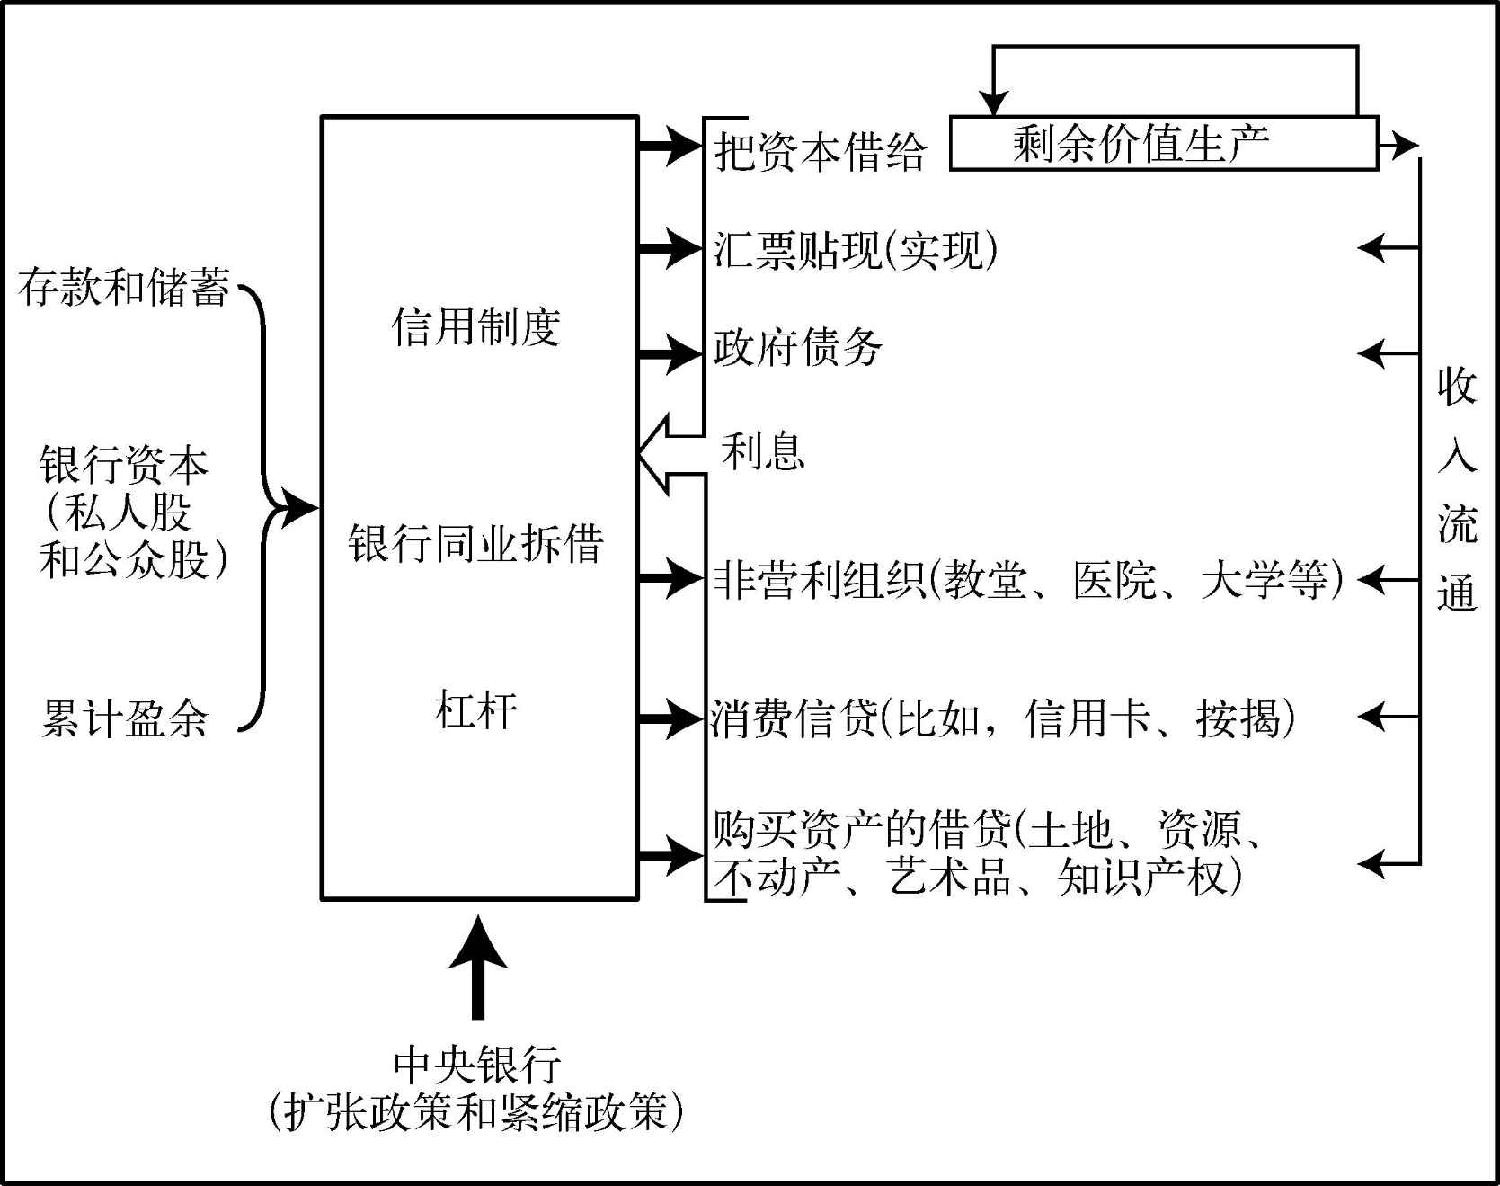
\includegraphics[scale=0.3]{david5.jpg}
\caption{生息资本的横向流通}
\label{fig:david5}
\end{figure}

货币借出的形式:
\begin{enumerate}
\item 借贷资本

  货币借给生产者,用来购买从事剩余价值生产所需要的不变资本和可变资本。……这些借
  出的货币用来进行实际的价值和剩余价值生产。其中没有任何虚拟的东西(尽管所有这种
  投资从定义来说无疑都具有投机性)。然而,当货币以发行股票的方式取得时,事情看起
  来有些不同。股票实际上是一种附属于纯粹的货币所有权的财产权。它实际上是对未来剩
  余价值生产的一个份额的法定索取权。

股票与证券是一种虚拟资本的形式,但是它们的虚拟特征因为与价值和剩余价值生产依然保持的宽松联系而得到缓解(用货币术语来说,企业收益支撑了股票价值)。然而,像安然那样的公司,虽然股票价格很高,并没有剩余价值被实际生产出来。它公布的收益是欺骗性的。

\item 用于价值实现的借贷

  货币可以被借出去实现已经生产出的商品的价值(甚至是还没生产出的,正如还没收割的农作物或将要建的房屋)。贴现率等同于那些将来某天到期的汇票的利息率。

 \item 政府借贷和国债

   政府可以凭借它获取收入(通过税费)的能力借到资本。它承诺将预期未来收益的一部分
   作为一笔资本的回报。政府债务的证书在借到的货币花光很久以后都能交易。大部分政府
   花费的货币与剩余价值生产几乎没有或完全没有直接的关系(尽管它经常通过形成一个可
   行的市场而发展出间接的关系,比如,军事装备)。这是\textbf{最卓越的虚拟资本}。
   政府一般不生产价值或剩余价值(例如,它维持君主制和打仗)。收入税被转化为源源不
   断的利息支付,它可以被资本化为一个总额,从而作为对未来收入的索取权进行交易。政
   府支出的一些类别确实和剩余价值生产相关。存在政府运营的企业(这些企业在世界许多
   地方都很重要,直到大约1980年后的新自由主义私有化浪潮的兴起,但它们在中国仍然很
   重要)。尽管这些企业不一定要获得利润,但它们以更低的成本向其他企业提供投入,这
   影响了整体的利润率。政府也投资于生产所必需的基础设施建设(高速公路、公共设施、
   排污和供水等等)。\textbf{它可以提供这些不变资本投入,只要求利息作为回报,因此
     有助于缓解任何利润率下降的趋势。}比如,债务融资的“生产性政府支出”这个范畴
   早在豪斯曼男爵重建第二帝国巴黎的基础设施时就变得极为重要了。但是大多数的政府债
   务是纯粹虚拟的。(Big Note)

\item 非营利组织的借贷

  包括私立医院、大学、教堂、博物馆和各类文化机构。对它们的借贷属于\textbf{虚拟资
    本的范畴,}因为他们多半不生产价值或剩余价值(尽管一些大学和医院的分支机构通过
  创新和研究直接涉及剩余价值生产)。用于支付借贷利息的收入有各种来源,但在我们的
  时代主要是依靠\textbf{使用费和捐赠}。

  \item 消费者信贷

    迄今为止,美国最重要的消费者信贷形式是房地产抵押贷款,马克思明确将其列为虚拟
    资本形式的一种。尽管家中没有发生直接的价值或剩余价值生产,家务劳动在确定劳动
    力价值方面的作用显著影响了剩余价值的生产。消费者信贷现在蕴藏着巨大的商机,它
    在管理经济中的总需求和为“\textbf{第二级的剥削形式}”提供充足机会中起了关键作
    用。马克思偶尔承认这种“第二级的剥削形式”,但一般将其作为边缘形式而不考虑。(Note)
   \item 为了取得和购买资产及其他索取收入的纸质证书而进行的借贷(比如自然资源的特许权、专利、土地和房产的租金)

\end{enumerate}

\bigskip
资产市场(从艺术投资到土地和资源买卖的所有事物)的扩散已经成为近来资本主义历史上的显著特征。大量过剩的货币经营资本涌向这些市场。


银行家一般不歧视(尽管他们可能会专门化)这些不同的借贷选择。他们的资本会流向任何
需求、回报率和安全性最有利的地方,以及任何未来前景看起来最光明的地方。\textbf{预
  期}——对未来的信念——在这些市场的运转中发挥了主导性作用。也存在这种可能,即一些投
资可能性被其他需求(和预期)更高的投资所“\textbf{挤出}”。(这是常见的对大规模政
府借贷或资产泡沫的批评:\textbf{它们挤出了对生产性活动的投资并增加了其他投资活动
  的利息成本。})(Big Note: 不理解这句话)

在生息货币资本的流动中,不平衡会频繁发生。恰恰因为这些资本是独立的、自主的,它们
可以影响总体的资本主义发展的运动规律,同时自己周期性地单独酝酿一场危机。例如,如
果大量过剩的货币经营资本流入土地和房地产市场(正如发生在20世纪80年代的日本以
及2000年后的美国、西班牙、爱尔兰等国的情况),那么,就会造成信用流通的巨大扭曲和
资产价值的投机性繁荣,直到崩溃发生并进行强制纠正。(Big Note)

即使在泡沫状况还不明显的时候,美国采取了许多措施把信用扩张到房屋所有权。这是资本从一般消费者,特别是从劳动者那里重获财富的主要方式。(Big Note)

\begin{quotation}
  资本的现实积累的标志,即规模扩大的再生产的标志,又在什么程度上不是这种标志呢?
  所谓资本过剩(plethora),一个始终只用于生息资本即货币资本的用语,仅仅是表现产
  业生产过剩的一个特殊方式呢,还是除此以外形成的一种特殊的现象呢?这种过剩即货币
  资本的供给过剩,是否与停滞的货币总量(金银条块、金币和银行券)的存在相一致,从
  而现实货币的这种过剩,是否就是借贷资本的上述过剩的反映和表现形式
  呢?

货币紧迫,即借贷资本不足,又在什么程度上反映出现实资本(商品资本和生产资本)的不
足呢?另一方面,它又在什么程度上与货币本身的不足,即流通手段的不足相一致呢?\pagescite[][539]{capital3}
\end{quotation}

再一次用当代的说法,货币供给收缩和银行间信贷的冻结是由中央银行和国家权力机关施加的金融收缩的信号吗?还是缺乏有利可图的投资机会的信号?(Big Note)

这背后有一个更一般的问题:债务的积累和财富的积累在什么程度上是有关联的?这是虚拟
资本形式的增殖所提出的问题。比如,“国债资本的积累,不过是表明国家债权人阶级的增
加,这个阶级有权把税收中的一定数额预先划归自己所有”。因此,“连债务积累也能表现
为资本积累”。\pagescite[][540]{capital3} 但是,像往常一样,“表现”这个词标志着
在拜物教面具的背后很可能有别的事情正在发生。发生了什么呢?问题是国债(虚拟资本)
积累可以转化为实际的货币资本,从而使虚拟资本变成现实资本。但这假定了国债是可以交
易的。这反过来意味着虚拟资本继续和以前一样流通。股票和有价证券也是如此,它们
是“不存在的资本的名义代表”:

\begin{quotation}
当这些证券的积累表示铁路、矿山、汽船等等的积累时,它们也表示现实再生产过程的扩大,就像动产征税单的扩大表示这种动产的增加一样。但是,作为纸制复本,这些证券只是幻想的,它们的价值额的涨落,和它们有权代表的现实资本的价值变动完全无关,尽管它们可以作为商品来买卖,因而可以作为资本价值来流通。\pagescite[][540-541]{capital3} 

\end{quotation}

当按揭贷款打包成为债务抵押债券时,它们似乎以过去的两倍的虚拟状态存在;但是当对冲基金经理把它们卖给毫不怀疑的、轻信的投资者并出色地赚了十亿时,很遗憾,他获得了一点都不虚幻的实际货币权力。


\begin{quotation}
  由这种所有权证书的价格变动而造成的盈亏,以及这种证书在铁路大王等人手里的集中,
  就其本质来说,越来越成为赌博的结果。赌博已经取代劳动,表现为夺取资本财产的本来
  的方法,并且也取代了直接的暴力……这种想象的货币财产,不仅构成私人货币财产的很
  大的部分,并且正如我们讲过的,也构成银行家资本的很大的部分。(Big Big Note)

  ……整个信用制度的惊人的扩大,总之,全部信用,都被他们当作自己的私有资本来利用。
  这些人总是以货币的形式或对货币的直接索取权的形式占有资本和收入。这类人的财产的
  积累,可以按极不同于现实积累的方向进行,但是无论如何都证明,他们攫取了现实积累
  的很大一部分。\pagescite[][541]{capital3}

  只要再生产过程顺畅地进行,从而资本回流确有保障,这种信用就会持续下去和扩大起来,
  并且它的扩大是以再生产过程本身的扩大为基础的。一旦由于回流延迟,市场商品过剩,
  价格下降而出现停滞,产业资本就会过剩,不过这种过剩是在产业资本不能执行自己的各
  种职能的形式上表现出来的。有大量的商品资本,但卖不出去。有大量的固定资本,但由
  于再生产停滞,大部分闲置不用。(Note: 马克思对周期的一个描述)\pagescite[][546-547]{capital3} 

  一旦新的危机爆发,信用突然停止,支付停滞,再生产过程瘫痪……在借贷资本几乎绝对
  缺乏的同时,闲置的产业资本发生过剩。
\end{quotation}

借贷资本的积累可以从正常资本的积累中“沉淀下来”。“在现实积累不断扩大时,货币资
本积累的这种扩大,一部分是这种现实积累扩大的结果,一部分是各种和现实积累的扩大相
伴随但和它完全不同的要素造成的结果” ——比如,生产性公司的股票和证券价值上升——“一
部分甚至是现实积累停滞的结果”——过剩商品没有卖出去,但是它的贴现价值通过汇票实现
了。但“这种积累可以表示各种和现实积累很不相同的要素”——比如,资本化后上升的资产
价值、政府虚拟资本的形成或消费信贷。总结果就是“在周期的一定阶段出现货币资本的过
剩”。\pagescite[][574]{capital3}

随后信用就收缩,“(1) 因为这种资本闲置不用;(2) 因为再生产过程顺畅进行的信念已经遭到破坏;(3) 因为对这种商业信用的需求已经减少。”[43]信用的缺乏使得

\begin{quotation}
  通过信用来获得商品就比较困难……在危机中,因为每个人都要卖而卖不出去,但是为了
  支付,又必须卖出去,所以,正是在这个信用最缺乏的时刻,不是闲置的寻找出路的资本,
  而是停滞在自身的再生产过程内的资本的数量最大。这时,由于再生产过程的停滞,已经
  投入的资本实际上大量地闲置不用。工厂停工,原料堆积,制成的产品作为商品充斥市场。
  因此,如果把这种情况归因于生产资本的缺乏,那就大错特错了。正好在这个时候,生产
  资本是过剩了,无论就正常的、但是暂时紧缩的再生产规模来说,还是就已经萎缩的消费
  来说,都是如此。\pagescite[][574]{capital3}

\end{quotation}

“我们假定整个社会只是由产业资本家和雇佣工人构成”——撇开其他所有特征,比如价格波
动和信用制度所助长的买空卖空和投机交易。这样,

\begin{quotation}
  危机好像只能由各个不同部门生产的不平衡,由资本家自己的消费和他们的积累之间的不
  平衡来说明。然而实际情况是,投在生产上的资本的补偿,在很大程度上依赖于非生产阶
  级的消费能力;而工人的消费能力一方面受工资规律的限制,另一方面受以下事实的限制,
  就是他们只有在他们能够为资本家阶级带来利润时才能被雇佣。\textbf{一切现实的危机
    的最后原因,总是群众的贫困和他们的消费受到限制,而与此相对比的是,资本主义生
    产竭力发展生产力,好像只有社会的绝对的消费能力才是生产力发展的界
    限}。\pagescite[][574-578]{capital3}(Big Big Note)


\end{quotation}

这当然是最有名的论断之一(第二卷第351页也有),\textbf{和利润率下降是“现代政治经
  济学最重要的规律”这一断言一样,也需要结合上下文语境来理解。}对产业周期的研究表
明,这两种陈述之间并没有必然的对立。由于群众消费受到限制,利润率在短期内可能会下
降。这和第三卷前面章节中通常用来解释利润率下降的机制是非常不同的。但是解雇工人会
减少市场需求,使得商品卖不出去和生产能力闲置,从而诱发资本家减少工资并解雇更多的
工人。马克思清楚地看到了产业周期中这种螺旋式下跌的可能性。这是否形成了一个长期趋
势完全是另一个问题。信用制度允许资本摆脱这种直接的消费限制,至少在一段时间内是这
样的。“信用的最大限度,等于产业资本的最充分的运用……不顾消费界限”。在大
约1980年以后的工资压制的新自由主义时期,私人消费主要是通过扩展消费信贷来维持的。

马克思也观察到这种螺旋式下降在信用的帮助下如何可能\textbf{反转}过来。大量的闲置借
贷和货币资本——伴随着低利率——在危机后形成,并成为复苏的关键。“在危机以后的复苏时
期,人们要求借贷资本,却是为了购买,为了把货币资本转化为生产资本或商业资本。所以,
这时,要求借贷资本的,或者是产业资本家,或者是商人,产业资本家把借贷资本用于购买
生产资料和劳动力。”\pagescite[][580]{capital3} \textbf{低利率使对固定资本的长期
  投资和开启全新的事业看上去更有吸引力。}\pagescite[][553]{capital3} 在扩张的初始
阶段利率通常维持在较低水平,这时宽松信贷发挥着其最具有建设性的作用,而这有助于进
一步的扩张和世界市场的一体化,正如我们所见的。(Big Note: 当前的中国,是否是低利
息率呢?)
在他第一次试图解释周期性运动如何开展时,马克思写道:

\begin{quotation}
  如果再生产过程再一次达到过度紧张状态以前的那种繁荣局面,商业信用就会大大扩张,
  这种扩张实际上又是资本容易流回和生产扩大的“健全”基础。在这种情况下,利息率虽
  然已经高于最低限度,但是仍然很低……由于资本回流容易并且具有规则性,加上商业信
  用扩大,这就保证了借贷资本的供给(虽然需求已经增长),防止了利息率水平的上升。
  另一方面,只有到这时,没有准备资本甚至根本没有任何资本而完全依靠货币信用进行操
  作的冒险家们,才引人注目地涌现出来。此外,还有各种形式的固定资本的显著扩大和新
  型大企业的大批开张。现在,利息提高到它的平均水平。一旦新的危机爆发,信用突然停
  止,支付停滞,再生产过程瘫痪……在借贷资本几乎绝对缺乏的同时,闲置的产业资本发
  生过剩……这种产业周期的情况是,同样的循环一旦受到最初的推动,就必然会周期地再
  现出来。\pagescite[][553-554]{capital3} 

  
  在再生产过程的全部联系都是以信用为基础的生产制度中,只要信用突然停止,只有现金
  支付才有效,危机显然就会发生,对支付手段的激烈追求必然会出现。所以乍看起来,好
  像整个危机只表现为信用危机和货币危机。而且,事实上问题只是在于汇票能否兑换为货
  币。但是这种汇票多数是代表现实买卖的,而这种现实买卖的扩大远远超过社会需要的限
  度这一事实,归根到底是整个危机的基础。不过,除此以外,这种汇票中也有惊人巨大的
  数额,代表那种现在已经败露和垮台的纯粹投机营业;其次,代表利用别人的资本进行的
  已告失败的投机;最后,还代表已经跌价或根本卖不出去的商品资本,或者永远不会实现
  的资本回流。这种强行扩大再生产过程的全部人为体系,当然不会因为有一家像英格兰银
  行这样的银行,用它的纸券,给一切投机者以他们缺少的资本,并把全部已经跌价的商品
  按原来的名义价值购买进来,就可以医治好。并且,在这里,一切都以颠倒的形式表现出
  来,因为在这个纸券的世界里,在任何地方显现出来的都不是现实价格和它的现实要素,
  而只是金银条块、硬币、银行券、汇票、有价证券。在全国金融中心,例如伦敦,这种颠
  倒表现得尤为明显。全部过程都变为不可理解。\pagescite[][555]{capital3}


一切国家都会先后卷入危机……那时就会发现,一切国家,除了少数例外,出口和进口过多,
以致\textbf{支付差额对一切国家来说都是逆差},所以实际上问题并不在于支付差额的方面。例如英
国正苦于金的流出。它进口过多。但同时,所有别的国家堆积着过多的英国商品。所以它们
也进口过多或被输入过多。\pagescite[][556]{capital3} 

危机也许首先是在英国,在这个提供信用最多而接受信用最少的国家爆发,因为支付差
额……对它来说是逆差,尽管总的贸易额对它来说是顺差。……在英国以金的流出作为开端
并且伴随着这种流出而发生的崩溃,使英国的支付差额所以得到结清,部分地是由于英国进
口商人宣告破产……部分地是由于在国外廉价抛售一部分英国商品资本,部分地是由于出售
外国有价证券,买进英国有价证券等等。现在轮到另一个国家了。……1857年,美国爆发了
危机。于是金从英国流到美国。但是美国物价的涨风一停止,危机接着就在英国发生了。金
又由美国流到英国。英国和大陆之间也发生了同样的情况。在普遍危机的时刻,支付差额对
每个国家来说,至少对每个商业发达的国家来说,都是逆差,不过,这种情况,总是像排炮
一样,按照支付的序列,先后在这些国家里发生。\pagescite[][556-557]{capital3}(Big Big Note)

\end{quotation}

在马克思看来,“这个现象的普遍性恰好证明:(1) 金的流出只是危机的现象,而不是危
机的原因 (2) 金的流出现象在不同各国发生的顺序只是表明,什么时候会轮到这些国家算
总账,什么时候会轮到这些国家发生危机……”尽管马克思强调了普遍性,但这种集中
于“金的流出”的连续发生的事件只是现在危机采取的一种可能的地理形式。在我们的时代,
特别的是迅速增长的主权债务,比如希腊——部分产生于希腊为支付德国生产的商品而向德国
和法国银行进行的过量借贷。欧元的创造促进了这个过程。欧元使更有效率的生产者(德国)
受益,而破坏了南欧低效率的经济体的生产。结果是德国和法国银行持有的虚拟资本价值受
到威胁,这反过来威胁到法国的主权债务,甚至最终威胁到德国,除非整个欧元区协调行动。
结果证明在欧洲中央银行的“错误”章程下,协调行动特别困难。排炮,确实如此。(Note)

所有这些与信用市场相关的运动是容易察觉的。但是马克思不相信这些运动是危机的根源。根源在于资本过度积累的基本倾向和独立自主产生的过剩货币资本这两者的结合,而后者是出于自身利益堆积起来的。回想一下,

\begin{quotation}
仅仅由于这些和现实积累相独立、但和它相伴随的要素扩大了借贷资本的积累,就总会在周期的一定阶段出现货币资本的过剩;并且这种过剩会随着信用的发达而发展。因此,驱使生产过程突破资本主义界限的必然性,同时也一定会随着这种过剩而发展,也就是产生贸易过剩,生产过剩,信用过剩。同时,这种现象必然总是在引起反作用的各种形式上出现。\pagescite[][574]{capital3} 

\end{quotation}

我通常将这些组合称为“\textbf{过剩资本的处置问题}” 。资本过剩的趋势,特别是货币形式的资本
过剩的趋势,是所有危机的根源——这个论点值得探究。过剩资本很容易被吸收到虚拟资本形
成和流通的通道这个事实,成为既不能逃避也不能压制的中心问题——考虑到资本的货币形式
在货币资本家的绝对权力的支持下,在克服贮藏的必要性上发挥的积极作用。(Big Big Note)

第二三卷风格的差异,这种解释的问题在于:它和写作的年代是不一致的。第二卷的大部分内容是在完成第三卷的草稿后写的。因此,为什么马克思在写完关于商人资本和金融的激动人心和十分迷人的(尽管令人沮丧的是它不完整,而且有时前后不一致)材料后,在第二卷的论证中又回到枯燥的、技术性的叙述风格呢?


在这个背景下,他回到第二卷中资本内在本性的问题就说得通了。马克思寻找的是这种内在
本性的某种X射线,它能说明信用制度充满矛盾的颠倒错乱现象是如何以及为何会必然产生。
为什么资本根本的、潜在的矛盾总是采取金融和商业危机的形式呢?为了揭示所有问题的答
案,他在第二卷研究资本积累与流通时抛开了信用制度和生息资本的流通,以便于理解为什
么资本的流通和积累必然要求信用和“独立自主的”货币资本来发挥作用。总之,从第二卷
中我们理解了为什么资本在缺乏信用制度时无法生存,为什么财富积累和债务积累必然是同
步进行的,以及在一个资本主义剩余价值生产体系里,为什么价值和它的货币表现之间的中
心矛盾内化为供给和需求永远不会也必然不会相等的矛盾。在我看来,上面从第三卷第554页
引用的冗长段落,完全印证了这一点。

但是,如果我理解得没有错,第二卷的一个关键目标是深入剖析第三卷的金融章节中展现出
来的恶毒的拜物教,那么第二卷在马克思全部著作中的地位就重新确立了,理应得到更细致
深入的研究。马克思清楚地明白,他需要从流通的角度构建一个和他在第一卷中从生产的角
度构建的一样的,关于资本运动规律的有说服力的模型。悲剧的是他没有完成这项工作,并
且他在把生产和流通这两个视角综合为一个可行的整体之前,便过早离世了。



%%% Local Variables:
%%% mode: latex
%%% TeX-master: "../main"
%%% End:
